\documentclass [11pt,twoside]{article}
\usepackage[utf8]{inputenc}
\usepackage[T1]{fontenc}

\usepackage[english]{babel}

%For LaTex syntax checking without bilding .pdf file
\usepackage{syntonly}
%\syntaxonly

%Page margins, header and footer positions
\usepackage{geometry}
 \geometry{
 a4paper,
 total={210mm,297mm},
 left=25mm,
 right=25mm,
 top=30mm,
 bottom=25mm,
 headsep=7mm}

\interfootnotelinepenalty=10000

%paragraph spacing
\setlength{\parskip}{1em}
%avoid the paragraph spacing to be applied to the table of content, the list of figures and the list of tables
\AtBeginDocument{\addtocontents{toc}{\protect\setlength{\parskip}{0pt}}}
\AtBeginDocument{\addtocontents{lof}{\protect\setlength{\parskip}{0pt}}}
\AtBeginDocument{\addtocontents{lot}{\protect\setlength{\parskip}{0pt}}}

%for nice tables
\usepackage{booktabs}
\usepackage{array}
\newcolumntype{P}[1]{>{\raggedright\arraybackslash}p{#1}}
\usepackage{longtable} %multi-page tables
\usepackage{multirow}

%handling floats
\usepackage{placeins}

%for placements of floats in the [H] here position
\usepackage{here}

%titles font size
\usepackage{titlesec}
\titleformat*{\section}{\huge\bfseries}
\titleformat*{\subsection}{\LARGE\bfseries}
\titleformat*{\subsubsection}{\Large\bfseries}
\titleformat*{\paragraph}{\large\bfseries}
\titleformat*{\subparagraph}{\large\bfseries}

%footnotes
\usepackage{footnote}

%To display filling dots in the TOC for all entries
\usepackage[titles]{tocloft}
\renewcommand{\cftsecleader}{\cftdotfill{\cftdotsep}}

%Define new header and footer style
\usepackage{fancyhdr}

\pagestyle{fancy}
\fancyhf{}
\lhead{\color{Gray}{\small{Travlendar+ project by YOUR NAMES}}}
\lfoot{\textcolor{Gray}{\small{Copyright © 2017, YOUR NAMES – All rights reserved}}}
\rfoot{\textcolor{Gray}{\thepage}}
\renewcommand{\headrulewidth}{0pt}

%PACKAGES
\usepackage{wasysym}
\usepackage{pifont}

\newcommand{\supported}{\ding{52}\xspace}
\newcommand{\unsupported}{\ding{55}\xspace}
\newcommand{\partsupported}{\textcolor{black!40}{\ding{52}}\xspace}
\newcommand{\lowsupported}{\textcolor{black!20}{\ding{52}}\xspace}
\newcommand{\unknowsupported}{\textbf{?}\xspace}

%Font: Times
\usepackage{times}
%Change monospaced font
\renewcommand{\ttdefault}{lmtt}

%tables
\usepackage{tabu}
\usepackage{tabularx}
\usepackage{ltablex}
\usepackage{longtable}
\usepackage{float} % To allow the use of H modifier in long tables

%landscape mode
\usepackage{pdflscape}
\usepackage{rotating}
\usepackage{caption}

%make landscape mode be sensitive to even and odd pages
%start
\def\myrotate{\ifodd\c@page\else-\fi 90}
\makeatletter
\global\let\orig@begin@landscape=\landscape%
\global\let\orig@end@landscape=\endlandscape%
\gdef\@true{1}
\gdef\@false{0}
\gdef\landscape{%
    \global\let\within@landscape=\@true%
    \orig@begin@landscape%
}%
\gdef\endlandscape{%
    \orig@end@landscape%
    \global\let\within@landscape=\@false%
}%
\@ifpackageloaded{pdflscape}{%
    \gdef\pdf@landscape@rotate{\PLS@Rotate}%
}{
    \gdef\pdf@landscape@rotate#1{}%
}
\let\latex@outputpage\@outputpage
\def\@outputpage{
    \ifx\within@landscape\@true%
        \if@twoside%
            \ifodd\c@page%
                \gdef\LS@rot{\setbox\@outputbox\vbox{%
                    \pdf@landscape@rotate{-90}%
                    \hbox{\rotatebox{90}{\hbox{\rotatebox{180}{\box\@outputbox}}}}}%
                }%
            \else%
                \gdef\LS@rot{\setbox\@outputbox\vbox{%
                    \pdf@landscape@rotate{+90}%
                    \hbox{\rotatebox{90}{\hbox{\rotatebox{0}{\box\@outputbox}}}}}%
                }%
            \fi%
        \else%
            \gdef\LS@rot{\setbox\@outputbox\vbox{%
                \pdf@landscape@rotate{+90}%
                \hbox{\rotatebox{90}{\hbox{\rotatebox{0}{\box\@outputbox}}}}}%
            }%
        \fi%
    \fi%
    \latex@outputpage%
}
\makeatother
%end

%graphics
\usepackage{graphicx}
\usepackage[dvipsnames, table]{xcolor}
%If you upload images from PC, you need to insert code for the path here (different for Windows and Unix OS)

%References
%\usepackage{xpatch}
%\usepackage[backend=biber, style=numeric, citestyle=numeric, sorting=none]{biblatex}
%\addbibresource{main.bib}

%Other
\usepackage{ifthen}
\usepackage{xspace}
\usepackage{enumitem}
\usepackage{amssymb}
\usepackage[pdftex, colorlinks]{hyperref}
%prevents internal hyperlinks default color (red), keeps links active but black
\hypersetup{%
  colorlinks = true,
  linkcolor  = black
}
\newcommand{\comment}[1]{{\color{Red}$\blacktriangleright$ Comment: #1 $\blacktriangleleft$}}


% Some utilities\ldots
\usepackage{soul}
\usepackage{tikz}

\usetikzlibrary{calc}
\usetikzlibrary{decorations.pathmorphing}


\makeatletter

\newcommand{\defhighlighter}[3][]{%
  \tikzset{every highlighter/.style={color=#2, fill opacity=#3, #1}}%
}

\defhighlighter{yellow}{.5}

\newcommand{\highlight@DoHighlight}{
  \fill [ decoration = {random steps, amplitude=1pt, segment length=15pt}
        , outer sep = -15pt, inner sep = 0pt, decorate
       , every highlighter, this highlighter ]
        ($(begin highlight)+(0,8pt)$) rectangle ($(end highlight)+(0,-3pt)$) ;
}

\newcommand{\highlight@BeginHighlight}{
  \coordinate (begin highlight) at (0,0) ;
}

\newcommand{\highlight@EndHighlight}{
  \coordinate (end highlight) at (0,0) ;
}

\newdimen\highlight@previous
\newdimen\highlight@current

\DeclareRobustCommand*\highlight[1][]{%
  \tikzset{this highlighter/.style={#1}}%
  \SOUL@setup
  %
  \def\SOUL@preamble{%
    \begin{tikzpicture}[overlay, remember picture]
      \highlight@BeginHighlight
      \highlight@EndHighlight
    \end{tikzpicture}%
  }%
  %
  \def\SOUL@postamble{%
    \begin{tikzpicture}[overlay, remember picture]
      \highlight@EndHighlight
      \highlight@DoHighlight
    \end{tikzpicture}%
  }%
  %
  \def\SOUL@everyhyphen{%
    \discretionary{%
      \SOUL@setkern\SOUL@hyphkern
      \SOUL@sethyphenchar
      \tikz[overlay, remember picture] \highlight@EndHighlight ;%
    }{%
    }{%
      \SOUL@setkern\SOUL@charkern
    }%
  }%
  %
  \def\SOUL@everyexhyphen##1{%
    \SOUL@setkern\SOUL@hyphkern
    \hbox{##1}%
    \discretionary{%
      \tikz[overlay, remember picture] \highlight@EndHighlight ;%
    }{%
    }{%
      \SOUL@setkern\SOUL@charkern
    }%
  }%
  %
  \def\SOUL@everysyllable{%
    \begin{tikzpicture}[overlay, remember picture]
      \path let \p0 = (begin highlight), \p1 = (0,0) in \pgfextra
        \global\highlight@previous=\y0
        \global\highlight@current =\y1
      \endpgfextra (0,0) ;
      \ifdim\highlight@current < \highlight@previous
        \highlight@DoHighlight
        \highlight@BeginHighlight
      \fi
    \end{tikzpicture}%
    \the\SOUL@syllable
    \tikz[overlay, remember picture] \highlight@EndHighlight ;%
  }%
  \SOUL@
}

\makeatother

% Common abbrev. are set as commands to ensure proper spacing after the dot
\RequirePackage{xspace}
\newcommand{\ie}{i.e.\@\xspace}
\newcommand{\aka}{a.k.a.\@\xspace}
\newcommand{\Ie}{I.e.\@\xspace}
\newcommand{\cf}{cf.\@\xspace}
\newcommand{\Cf}{Cf.\@\xspace}
\newcommand{\eg}{e.g.\@\xspace}
\newcommand{\Eg}{E.g.\@\xspace}
\newcommand{\etal}{et al.\@\xspace}
\newcommand{\etc}{etc.\@\xspace}
\newcommand{\wrt}{w.r.t.\@\xspace}
\newcommand{\Wrt}{W.r.t.\@\xspace}



\date{}


\begin{document}
        %TITLE PAGE
        \begin{titlepage}
                %LOGO
                {\begin{table}[t!]
                \centering
                \begin{tabu} to \textwidth { X[1.3,r,p] X[1.7,l,p] }
                \textcolor{Blue}
                {\textbf{\small{Travlendar+ project YOUR NAMES}}} & 
\includegraphics[scale=0.5]{Images/PolimiLogo}
                \end{tabu}
                \end{table}}~\\ [7cm]

                %TITLE 
                \begin{flushleft}
                %Replace the text string with your title
                {\textcolor{Blue}{\textbf{\Huge{Requirement Analysis and Specification Document}}}} \\ [1cm]
                \end{flushleft}
        \end{titlepage}

        %Define deliverable specific info
        %Replace cell contents where needed
        \begin{table}[h!]
                \begin{tabu} to \textwidth { X[0.3,r,p] X[0.7,l,p] }
                \hline
                
                \textbf{Deliverable:} & RASD\\
                \textbf{Title:} & Requirement Analysis and Verification Document \\
                \textbf{Authors:} & YOUR NAMES \\
                \textbf{Version:} & 1.0 \\ 
                \textbf{Date:} & 31-January-2016 \\
                \textbf{Download page:} & LINK TO YOUR REPOSITORY \\
                \textbf{Copyright:} & Copyright © 2017, YOUR NAMES – All rights reserved \\
                \hline
                \end{tabu}
        \end{table}

        \setcounter{page}{2}
        %------------------------------------------------------------------------------------------------------------------------------------------------
        \newpage
        \addcontentsline{toc}{section}{Table of Contents}
        \tableofcontents
        \newpage
        \addcontentsline{toc}{section}{List of Figures}
        \listoffigures
        \addcontentsline{toc}{section}{List of Tables}
        \listoftables
        %------------------------------------------------------------------------------------------------------------------------------------------------
        \clearpage
        \section{Introduction}
\label{sect:introduction}

\subsection{Purpose}
\label{subsect:purpose}

This section should include the goals.

This document represents the Requirement Analysis and Specification Document (RASD). Goals of this document are to completely describe the system in terms of functional and non-functional requirements, analyze the real needs of the customer in order to model the system, show the constraints and the limit of the software and indicate the typical use cases that will occur after the release. This document is addressed to the developers who have to implement the requirements and could be used as a contractual basis

\subsection{Scope}
\label{subsect:scope}

Scope: here we include an analysis of the world and of the shared phenomena. Identifies the product and application domain.

\subsubsection{Description of the given problem}
\label{subsect:descriptionofthegivenproblem}

In these trying times of global pandemic, such as a common matter as going grocery shopping has become a relevant threat for the general public health. In spite of this situation, grocery shopping still remains an essential need which has to be carried out: being so, avoiding crowding up either inside and outnside of grocery shops in order to avoid any source of hazards becomes the new main issue to focus on.\ CLup is a new software application that proposes itself to help either the grocery shop owners to adequate to the new governamental rules and grocery shop customers to protect their own health.\ Clup provides three main functionalities: a virtual queue, which has the conceptual purpose of substituing the physical lines outside of shops; a QR code identification system, which allows grocery shops managers to constantly monitor the influx of incoming people in the shop and, finally, the functionality of booking your grocery shop session on an online facility, this offers a further way to regulate people flow to shops managers and the possibility to better schedule their time to cutomers.

\subsubsection{Goals}
\label{subsect:goals}

Allow a manager to monitor the influx of clients in their store 
allow a manager to register his store on the system
Allow a customer to access a store with a QR code

Allow customers to line up in a virtual queue in order to access a grocery shop
allow a manager to get a numbered ticket to a client that represents their place in the queue
allow a customer to get a numbered ticket that represents their place in the queue

Allow a customer to book a visit
Allow users to indicate the categories of items that they intend to buy;
Allow users to indicate the time they intend to go grocery shopping
Allow users to indicate the estimated permanence time 

\subsection{Phenomena}
\label{subsect:phenomena}

The machine: the portion of system to be developed.
The world (a.k.a. the environment): the portion of the real-world affected by the machine.
Requirements engineering is concerned with phenomena occurring in the world, as opposed to phenomena occurring inside the machine.

Goals are prescriptive assertions formulated in terms of \textbf{world} phenomena (not necessarily shared).

Domain properties/assumptions are descriptive assertions assumed to hold in the \textbf{world}.

Requirements are prescriptive assertions formulated in terms of \textbf{shared} phenomena.

Requirements are a bridge from the \textbf{machine} to the real \textbf{world}.

Find all the possible phenomena, than, for each one specify if its shared or not and who controls it (world or machine)

\subsubsection{World phenomena}
\label{subsubsect:worldphenomena}

World phenomena are phenomena that the machine can not observe.

\subsubsection{Shared Phenomena}
\label{subsubsect:sharedphenomena}

Some world phenomena are shared with the machine.
Shared phenomena can be controlled by the world and observed by the machine, or controlled by the machine andd observed by the world.

\subsection{Definitions, acronyms and abbreviations}
\label{subsect:definitionsacronymsabbreviations}

\subsubsection{Definitions}
\label{subsect:definitions}

\subsubsection{Acronyms}
\label{subsect:acronyms}

\subsubsection{Abbreviations}
\label{subsect:abbreviations}

\subsection{Revision history}
\label{subsect:revisionhistory}

\subsection{References}
\label{subsect:references}

\subsection{Overview}
\label{subsect:overview}

Describes contents and structure of the remainder of the RASD
        %------------------------------------------------------------------------------------------------------------------------------------------------
        \clearpage
        \section{Overall description}
\subsection{Product perspective}
\subsection{Product functions}
\subsection{User characteristics}
\subsection{Assumptions, dependencies and constraints}
        %------------------------------------------------------------------------------------------------------------------------------------------------
        \clearpage
        \section{Specific requirements}
\subsection{External interface requirements}
\subsubsection{User interfaces}
\subsubsection{Hardware interfaces}
\subsubsection{Software interfaces}
\subsubsection{Communication interfaces}
\subsection{Functional requirements}
\subsection{Performance requirements}
\subsection{Design constraints}
\subsubsection{Standards compliance}
\subsubsection{Hardware limitations}
\subsubsection{Any other contraint}
\subsection{Software system attributes}
\subsubsection{Reliability}
\subsubsection{Availability}
\subsubsection{Security}
\subsubsection{Mantainability}
\subsubsection{Portability}
        %------------------------------------------------------------------------------------------------------------------------------------------------
        \clearpage
        {\color{Blue}{\section{Overall Description}}}
        \label{sect:overview}
        Here you can see how to include an image in your document.

\begin{sidewaysfigure}
\centering
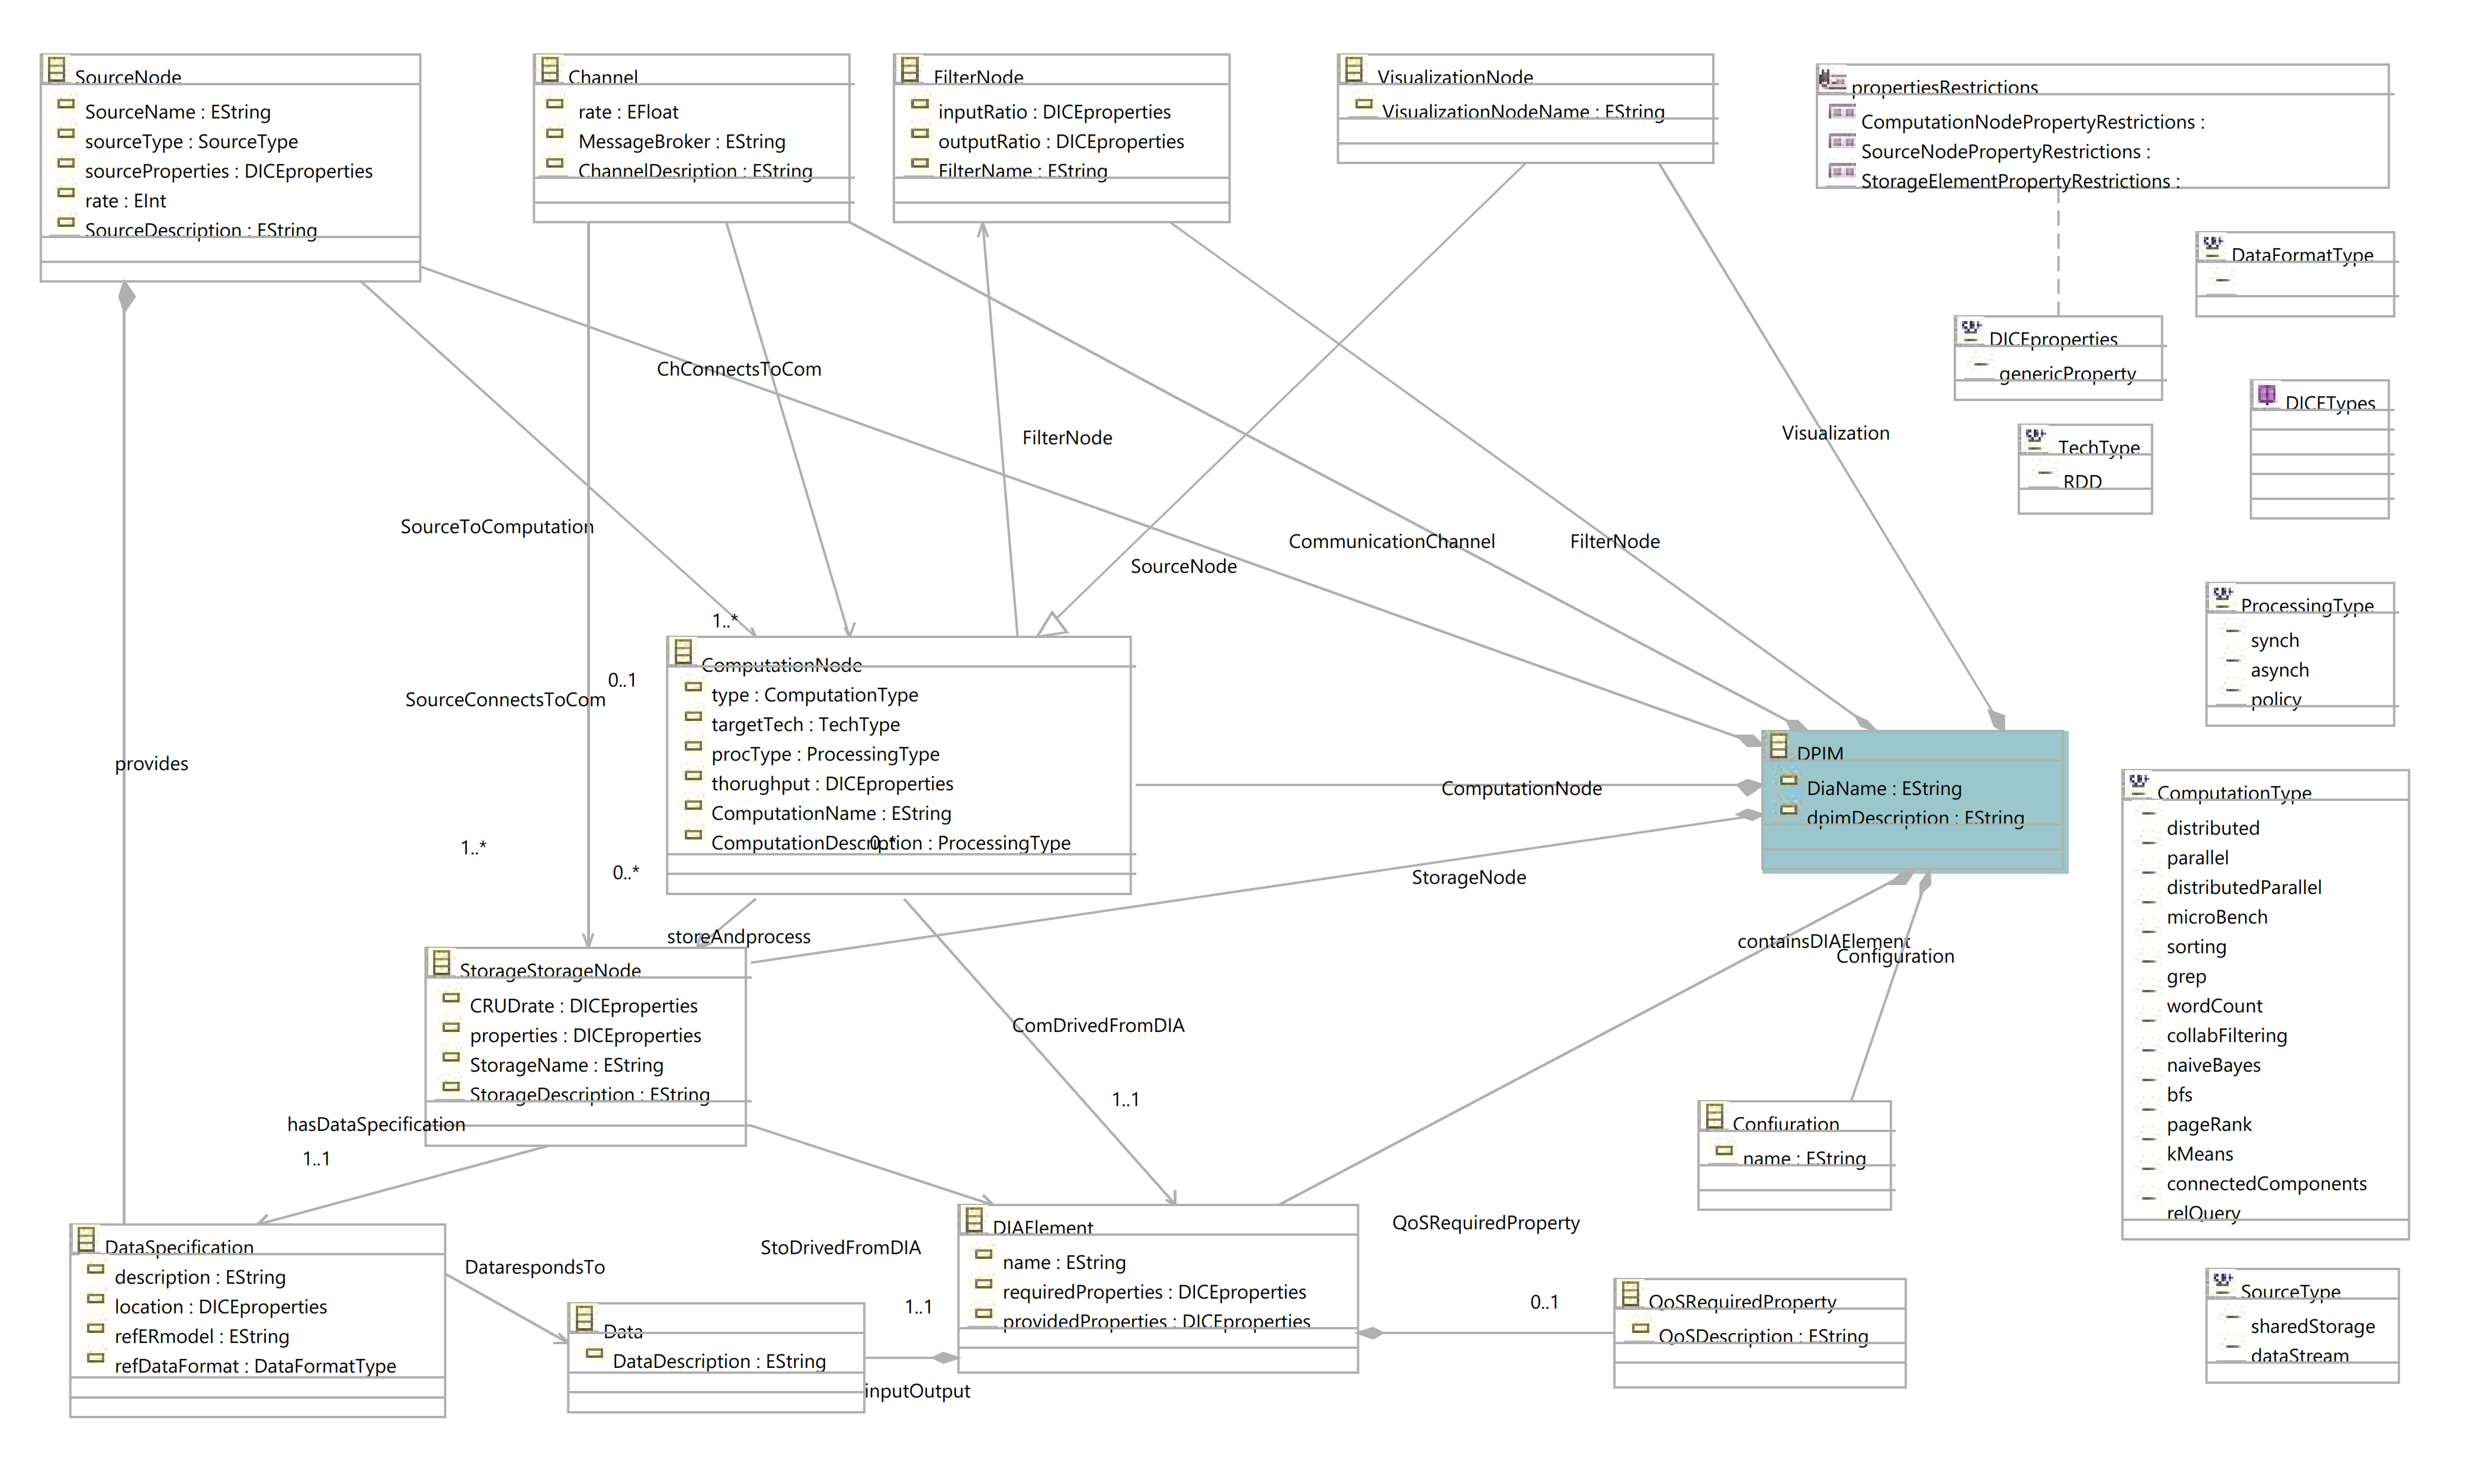
\includegraphics[width=\textwidth]{Images/11.png}
\caption{\label{fig:metamodel}DICE DPIM metamodel.}
\end{sidewaysfigure}

\begin{figure}
\centering
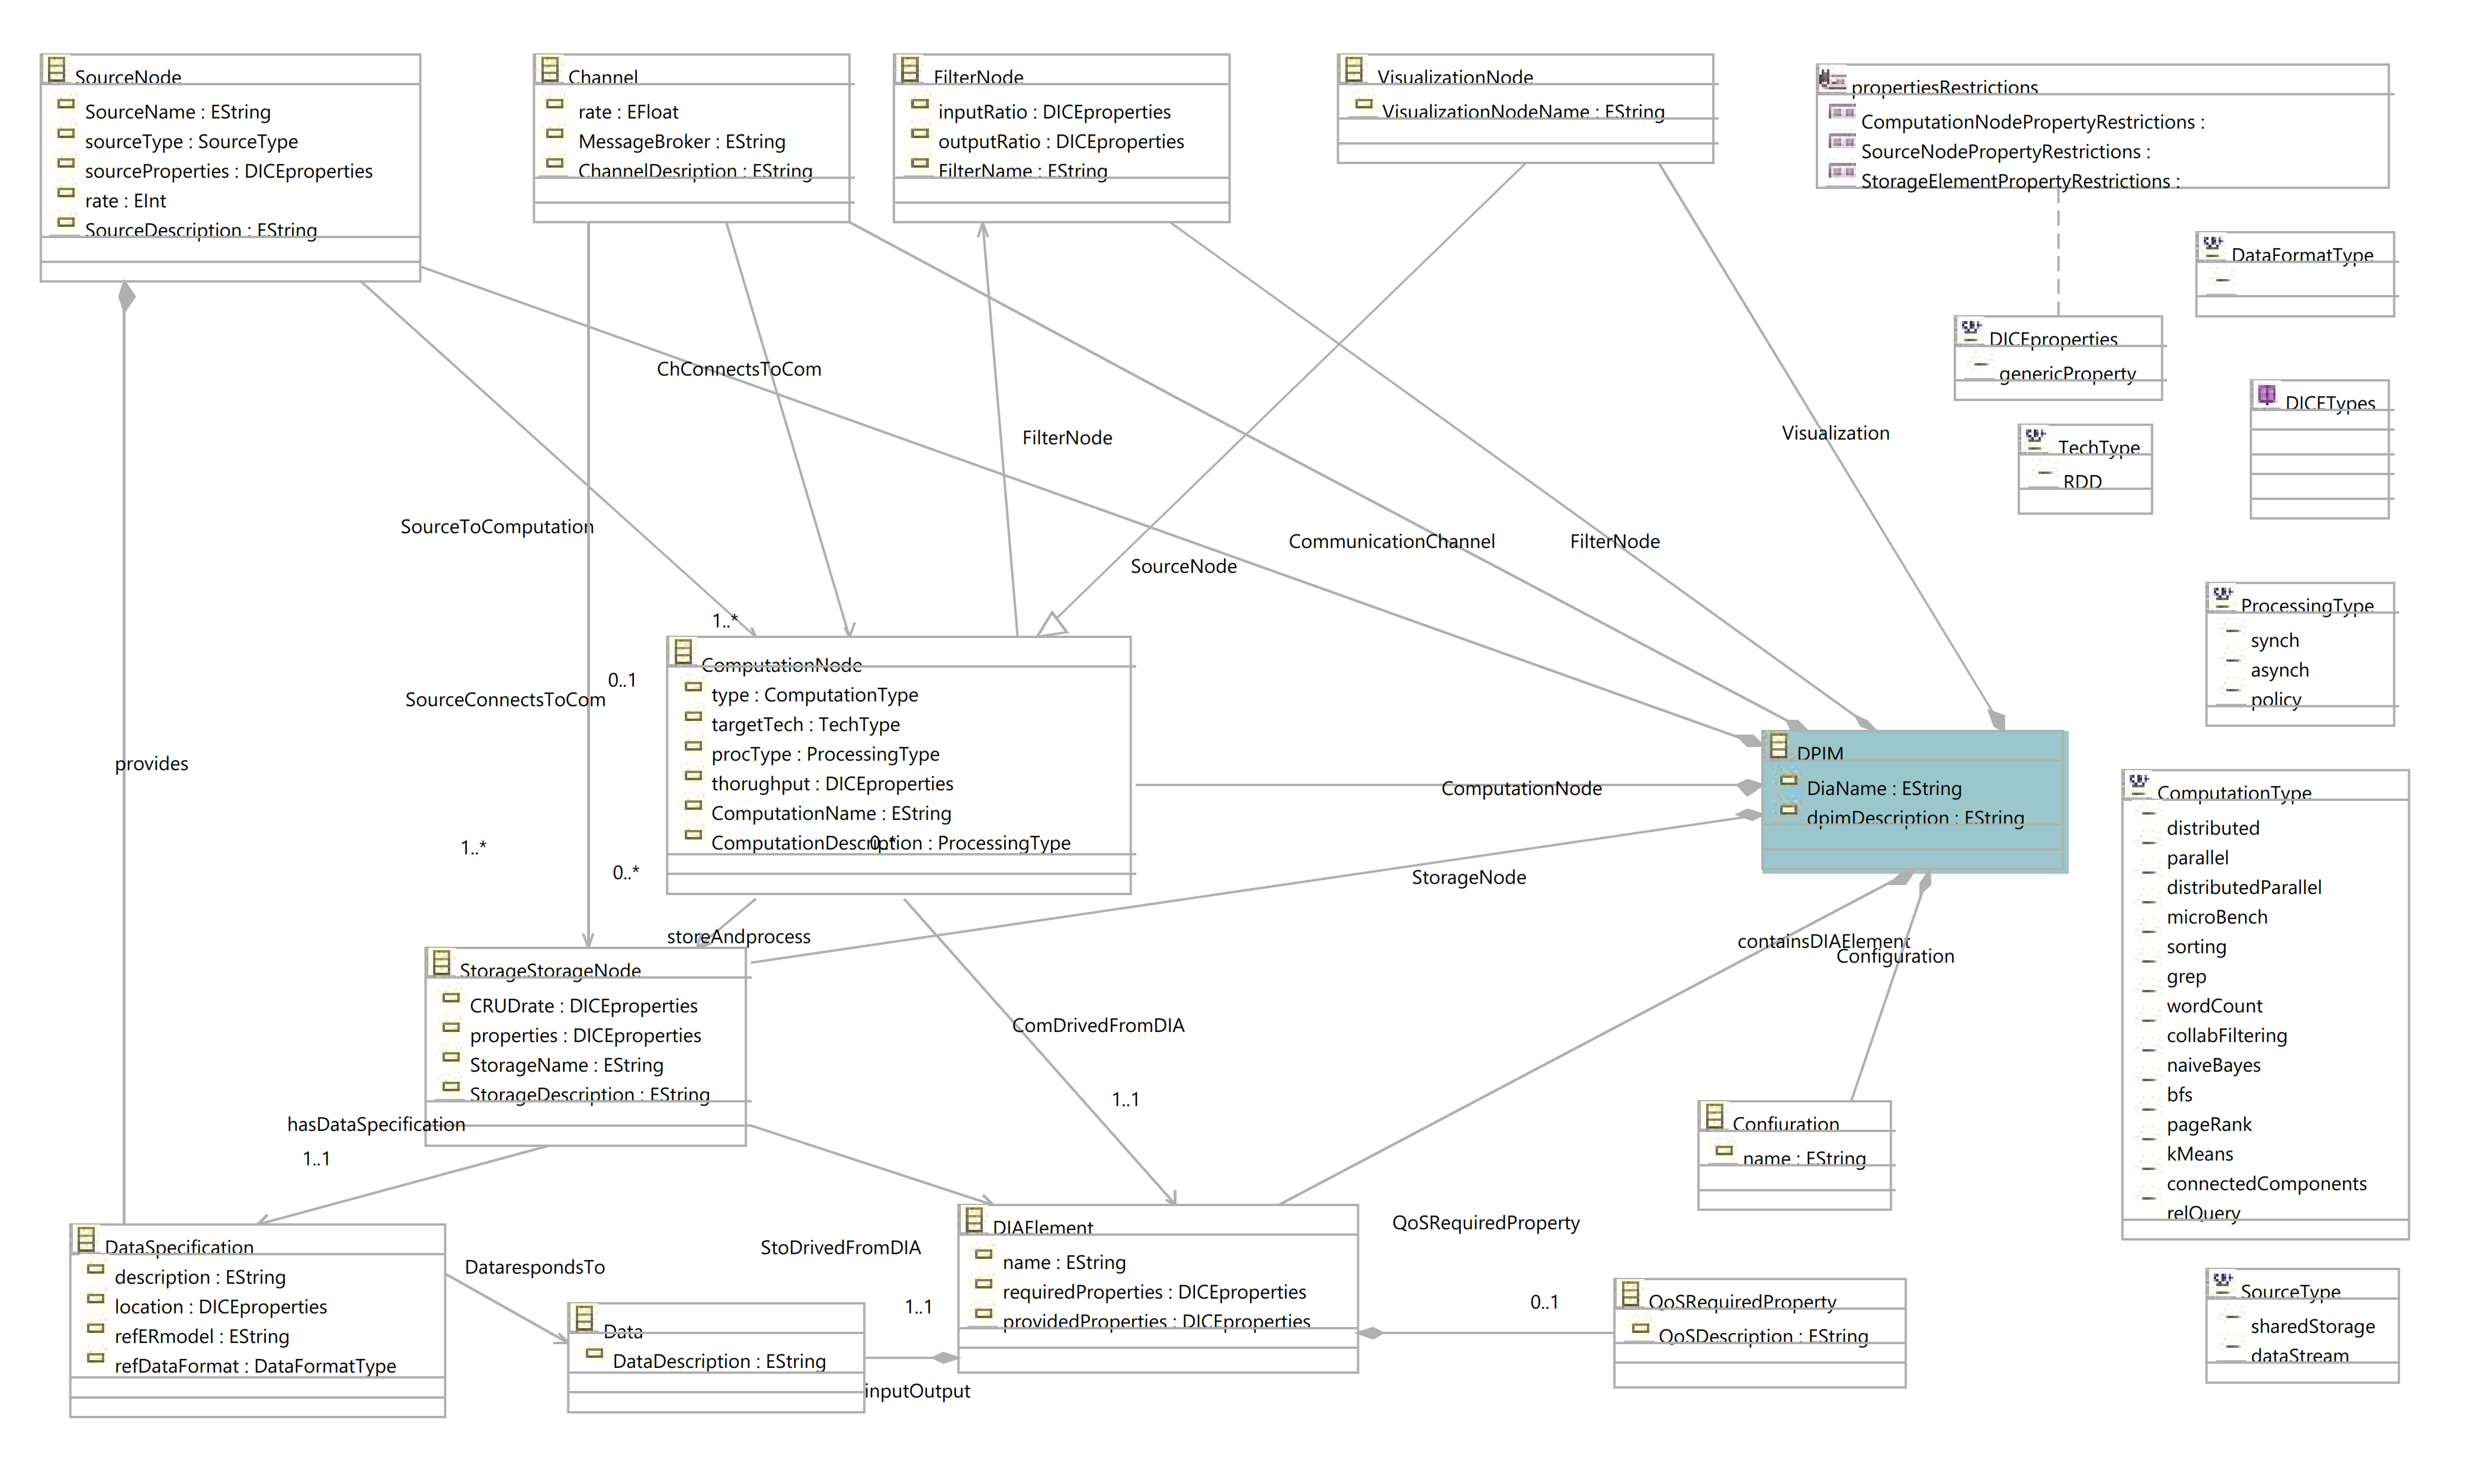
\includegraphics[width=\textwidth]{Images/11.png}
\caption{\label{fig:metamodel2}DICE DPIM metamodel in portrait form.}
\end{figure}

Here is the command to refer to another element (section, figure, table, ...) in the document: \emph{As discussed in Section~\ref{sect:overview} and as shown in Figure~\ref{fig:metamodel}, ...}. Here is how to introduce a bibliographic citation~\cite{DAM}. Bibliographic references should be included in a \texttt{.bib} file. 

Table generation is a bit complicated in Latex. You will soon become proficient, but to start you can rely on tools or external services. See for instance this \href{https://www.tablesgenerator.com}{https://www.tablesgenerator.com}. 

        %------------------------------------------------------------------------------------------------------------------------------------------------
        \clearpage
        {\color{Blue}{\section{Specific Requirements}}}
        \label{sect:requirements}
        Organize this section according to the rules defined in the project description. 

        %------------------------------------------------------------------------------------------------------------------------------------------------
        \clearpage
        {\color{Blue}{\section{Formal Analysis Using Alloy}}}
        \label{sect:alloy}
        Organize this section according to the rules defined in the project description. 

        %------------------------------------------------------------------------------------------------------------------------------------------------
        \clearpage
        {\color{Blue}{\section{Effort Spent}}}
        \label{sect:effort}
        Provide here information about how much effort each group member spent in working at this document. We would appreciate details here.

        %------------------------------------------------------------------------------------------------------------------------------------------------
        \clearpage
        \addcontentsline{toc}{section}{References}
        \bibliographystyle{plain}
        \bibliography{main}
        %------------------------------------------------------------------------------------------------------------------------------------------------
\end{document}
